\fontfamily{\sfdefault}\selectfont
% XCircuit output "rw_pn.tex" for LaTeX input from rw_pn.ps
\def\putbox#1#2#3#4{\makebox[0.00000in][l]{\makebox[#1][l]{}\raisebox{\baselineskip}[0.00000in][0.00000in]{\raisebox{#2}[0.00000in][0.00000in]{\scalebox{#3}{#4}}}}}
\def\rightbox#1{\makebox[0.00000in][r]{#1}}
\def\centbox#1{\makebox[0.00000in]{#1}}
\def\topbox#1{\raisebox{-0.60\baselineskip}[0.00000in][0.00000in]{#1}}
\def\midbox#1{\raisebox{-0.20\baselineskip}[0.00000in][0.00000in]{#1}}
   \scalebox{1}{
   \normalsize
   \parbox{2.66666in}{
   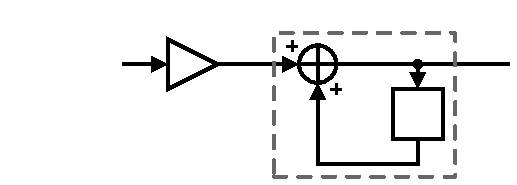
\includegraphics[scale=0.80000]{./figs/rw_pn.pdf}\\
   % translate x=924 y=776 scale 0.38
   \putbox{0.51200in}{0.71200in}{0.96}{w[n]}%
   \putbox{2.49600in}{0.72800in}{0.96}{y[n]}%
   \putbox{0.96000in}{0.79200in}{0.96}{\texttt{krw}}%
   \putbox{2.11200in}{0.32800in}{0.96}{$z^{-1}$}%
   \putbox{0.04800in}{0.51200in}{0.72}{...,+1,-1,-1,+1,...}%
   \putbox{1.83200in}{0.86400in}{0.96}{Integrator}%
   \putbox{1.19200in}{0.71200in}{0.96}{x[n]}%
   } % close 'parbox'
   } % close 'scalebox'
   \vspace{-\baselineskip} % this is not necessary, but looks better
\fontfamily{\rmdefault}\selectfont
